\section{Механизмы, поддерживающие высокую готовность}

\underline{Определение: } Высокая готовность (High Availability, HA) - это характеристика технической системы, разработанная для избежания невыполненного обслуживания путём уменьшения или управления сбоями и минимизации времени плановых простоев. 

Высокая готовность для каждой конкретной системы зависит от цели, для которой предназначена эта система. Для некоторых компаний высокая готовность значит максимальное downtime за год в несколько минут. Для других HA может значит downtime несколько часов в месяц.
Доступность(готовность) часто измеряется в <<Nines>>
\begin{figure}[h]
    \centering
    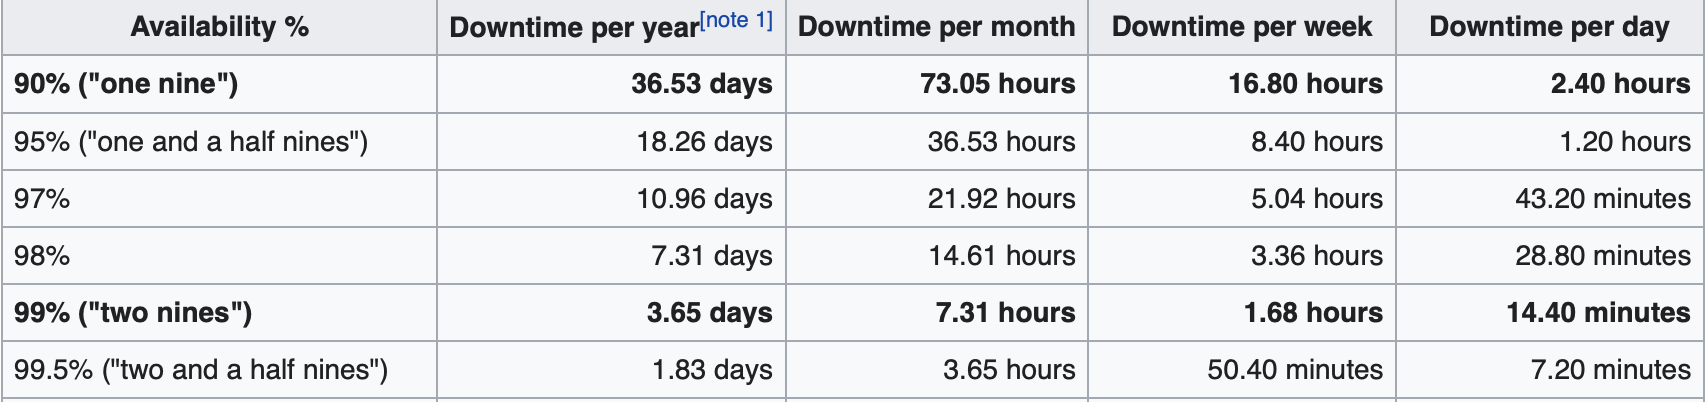
\includegraphics[width=0.8\textwidth]{database_protection-master/assets/avail.png}
    \caption{Пример Nines. Взято из википедии}
    \label{fig:mesh1}
\end{figure}

HA включает в себя несколько важных аспектов:
\begin{enumerate}
    \item Доступность данных 
    \item Защита данных
    \item Производительность
    \item Цена поддержки
\end{enumerate}
\subsection{Средства, поддерживающие высокую готовность}
\paragraph{Аппаратная и программная поддержки}
Существует несколько возможных уровней обеспечения высокой готовности системы: аппаратный и программный уровни. \\
\underline{Аппаратный уровень} включает в себя:
\begin{enumerate}
    \item \underline{Репликация БД}
    Репликация позволяет скопировать данные с одного сервера бд на другой.
    Существуют  два подхода репликации баз данных, рассмотрим каждый из них:
    \begin{itemize}
        \item \underline{Репликация Master-Slave} \\В этом подходе выделяется один основной сервер базы данных, который называется Мастером. На нем происходят все изменения в данных (любые запросы INSERT/UPDATE/DELETE). Слейв сервер постоянно копирует все изменения с Мастера. С приложения на Слейв сервер могут отправляться запросы на чтение данных (запросы SELECT). Таким образом Мастер сервер может отвечать за изменения данных, а Слейв за чтение. Также Мастер сервер может отвечать за все операции с данными, а Слейв являться бэкапом. При выходе из строя Слейва, достаточно просто переключить все приложение на работу с Мастером. После этого восстановить репликацию на Слейве и снова его запустить. Если выходит из строя Мастер, нужно переключить все операции (и чтения и записи) на Слейв. Таким образом он станет новым Мастером. После восстановления старого Мастера, настроить на нем реплику, и он станет новым Слейвом. Рассмотрена асинхронная репликация. При синхронной репликации результат сразу же записывается и в Мастер и в Слейв. Возвращение управления клиенту происходит только после записи в обе базы.
        \item \underline{Репликация Master-Master}\\ В этой схеме, любой из серверов может использоваться как для чтения так и для записи. При использовании такого типа репликации достаточно выбирать случайное соединение из доступных Мастеров. Вероятные поломки делают Master-Master репликацию непривлекательной. Выход из строя одного из серверов практически всегда приводит к потере каких-то данных. Последующее восстановление также сильно затрудняется необходимостью ручного анализа данных, которые успели либо не успели скопироваться.
    \end{itemize}

    Как уже говорилось ранее, репликацию данных можно разделить на синхронную и асинхронную. При асинхронной репликации изменения в slave или 2 master могут появляться с задержкой. При сихронной репликации может существовать только одна версия данных, что накладывает ограничения на работу с данными в процессе репликации.
        
    Существует логическая репликация. Логическая репликация — это метод репликации объектов данных и изменений в них, использующий репликационные идентификаторы (обычно это первичный ключ). Мы называем такую репликацию «логической», в отличие от физической, которая построена на точных адресах блоков и побайтовом копировании. PostgreSQL поддерживает оба механизма одновременно; Логическая репликация позволяет более детально управлять репликацией данных и аспектами безопасности. \\

    В логической репликации используется модель публикаций/подписок с одним или несколькими подписчиками, которые подписываются на одну или несколько публикаций на публикующем узле. Подписчики получают данные из публикаций, на которые они подписаны, и могут затем повторно опубликовать данные для организации каскадной репликации или более сложных конфигураций. \\

    Логическая репликация таблицы обычно начинается с создания снимка данных в публикуемой базе данных и копирования её подписчику. После этого изменения на стороне публикации передаются подписчику в реальном времени, когда они происходят. Подписчик применяет изменения в том же порядке, что и узел публикации, так что для публикаций в рамках одной подписки гарантируется транзакционная целостность. Этот метод репликации данных иногда называется транзакционной репликацией.
    
     \item \underline{RAID} - технология виртуализации данных для объединения нескольких физических дисковых устройств в логический модуль для повышения отказоустойчивости и производительности.
     Рассмотрим базовые уровни рейд массивов:
     \begin{enumerate}
         \item RAID 0 (striping — «чередование») — дисковый массив из двух или более жёстких дисков без резервирования.
         \item RAID 1 (mirroring — «зеркалирование») — массив из двух (или более) дисков, являющихся полными копиями друг друга. Не следует путать с массивами RAID 1+0 (RAID 10), RAID 0+1 (RAID 01), в которых используются более сложные механизмы зеркалирования.
         \item RAID 2. Массивы такого типа основаны на использовании кода Хэмминга. Диски делятся на две группы: для данных и для кодов коррекции ошибок, причём если данные хранятся на $2 ^ n - n - 1$ дисках, то для хранения кодов коррекции необходимо $n$ дисков. Суммарное количество дисков при этом будет равняться $2 ^ n - 1$. Данные распределяются по дискам, предназначенным для хранения информации, так же, как и в RAID 0, то есть они разбиваются на небольшие блоки по числу дисков. 
         \item В массиве RAID 3 из $n$ дисков данные разбиваются на куски размером меньше сектора (разбиваются на байты или блоки) и распределяются по $n - 1$ дискам. Ещё один диск используется для хранения блоков чётности. В RAID 2 для этой цели применялся $n - 1$ диск, но большая часть информации на контрольных дисках использовалась для коррекции ошибок «на лету», в то же время большинство пользователей устраивает простое восстановление информации в случае её повреждения, для чего хватает данных, умещающихся на одном выделенном жёстком диске. \\ Отличия RAID 3 от RAID 2: невозможность коррекции ошибок на лету.
         \item RAID 4 похож на RAID 3, но отличается от него тем, что данные разбиваются на блоки, а не на байты. Таким образом, удалось отчасти «победить» проблему низкой скорости передачи данных небольшого объёма. Запись же производится медленно из-за того, что чётность для блока генерируется при записи и записывается на единственный диск.
         \item RAID 5. Основным недостатком уровней RAID от 2-го до 4-го является невозможность производить параллельные операции записи, так как для хранения информации о чётности используется отдельный контрольный диск. RAID 5 не имеет этого недостатка. Блоки данных и контрольные суммы циклически записываются на все диски массива, нет асимметричности конфигурации дисков. Под контрольными суммами подразумевается результат операции XOR (исключающее или). Xor обладает особенностью, которая даёт возможность заменить любой операнд результатом, и, применив алгоритм xor, получить в результате недостающий операнд.
         \item RAID 6 — похож на RAID 5, но имеет более высокую степень надёжности — два (или более) диска данных и два диска контроля чётности. Основан на кодах Рида — Соломона и обеспечивает работоспособность после одновременного выхода из строя любых двух дисков. Обычно использование RAID 6 вызывает примерно 10-15 \% падение производительности дисковой группы, относительно RAID 5, что вызвано бо́льшим объёмом работы для контроллера (более сложный алгоритм расчёта контрольных сумм), а также необходимостью читать и перезаписывать больше дисковых блоков при записи каждого блока.
     \end{enumerate}
     Также существуют различные комбинации данных подходов.
\end{enumerate}
\underline{Программные подходы}:
\begin{enumerate}
    \item \underline{Автоматический перезапуск экземпляров БД, сетевых демонов и других ресурсов}
    \item \underline{Защита от повреждения данных(Data corruption protection)}
    \begin{itemize}
        \item Использование контрольных чек-сумм
        \item Автоматическое восстановление из резервной копии или повторная передача
    \end{itemize}
    \item \underline{PITR (Point In Time Recovery)} Данный механизм позволяет восстановить базу данных в том виде, в котором она была в каком-то моменте в прошлом.
    \item \underline{Application continuity (Oracle)} Маскирует от приложения и конечных пользователей падение базы данных и позволяет восстановить сеансы базы данных во время работы. 
    \item \underline{WAL} Данный подход будет описан ниже.
\end{enumerate}
\paragraph{Кластерная организация серверов баз данных} \\
Кластеризация базы данных - это процесс объединения нескольких серверов или инстансов, соединяющих одну базу данных. Иногда одного сервера может быть недостаточно для управления объемом данных или количеством запросов, тогда возникает необходимость в  кластере. 
 
 К общим требованиям, предъявляемым к кластерным системам, относятся:
\begin{enumerate}
    \item Высокая готовность
    \item Высокое быстродействие
    \item Масштабирование
    \item Удобство обслуживания
\end{enumerate}

Кластеры баз данных являются распространенной технологией.  Рассмотрим три типа архитектуры кластерных вычислений. Отказоустойчивые кластеры, высокопроизводительные кластеры и кластеры балансировки нагрузки.

\begin{enumerate}
\item Отказоустойчивые / высокодоступные кластеры. Кластер обеспечивает доступность сервиса путем репликации серверов и избыточной реконфигурации программного и аппаратного обеспечения. Таким образом, каждая система контролирует другую и работает на запросы, если какой-либо один из узлов выходит из строя.

\item Высокопроизводительные кластеры. Целью разработки высокопроизводительных кластеров баз данных является создание высокопроизводительных компьютерных систем. Основная цель - разумное распределение рабочей нагрузки.

\item Кластеры балансировки нагрузки. Эти кластеры базы данных служат для распределения нагрузки между различными серверами. Они стремятся обеспечить увеличенную пропускную способность сети, в конечном итоге увеличивая производительность. Системы в этой сети объединяют свои узлы, с помощью которых пользовательские запросы равномерно распределяются между участвующими узлами. 
\end{enumerate}

Несмотря на всю распределенную систему на заднем плане, пользователю это кажется единой системой. Использование кластеров варьируется от предприятия к предприятию, в зависимости от вида процессов и требуемого уровня производительности.
\paragraph{Параметры настройки СУБД} \\
Непонятно о чем это, настройки чего \\ 

\paragraph{Сохранение и восстановление БД} \\
Основным свойством транзакций СУБД является durability. Идея механизма обеспечения этого свойствая является одинаковой для всех СУДБ. СУБД использует специальный лог(Write-Ahead Lock - WAL), в который записываются все транзакции, результат которых не попал на физический диск. WAL — это журнал опережающей записи, технология, которую часто используют для улучшения надежности базы данных. Когда вы заносите информацию в базу данных, база выполняет несколько операций, манипулируя блоками.
Следовательно, с точки зрения файловой системы INSERT и UPDATE не являются атомарными операциями: если кто-то внезапно выключит ваш сервер, данные окажутся испорчены. Если возникает сбой, база данных использует этот файл для того, чтобы восстановить данные на момент падения. WAL — это бинарный лог, так что для его чтения нужна специальная утилита.
Например в PostreSQL данный файл называется WAL и лежит по пути \$PGDATA/pg\_xlog. 
PostgreSQL позволяет отключать WAL для отдельных таблиц, помечая их как UNLOGGED.

\subsection{Оперативное администрирование}
\paragraph{Задачи, средства и режимы администрирования}

Задачи администратора баз данных могут незначительно отличаться в зависимости от вида применяемой СУБД, но в основные задачи входит:
\begin{itemize}
    \item Проектирование базы данных.
    \item Оптимизация производительности базы данных.
    \item Резервирование и восстановление базы данных.
    \item Обеспечение целостности баз данных.
    \item Обеспечение перехода на новую версию СУБД.
\end{itemize}
Существуют различные программы и способы администрирования БД, которые напрямую зависят от БД. Основным инструментом работы с базой данных является DSL и программы, например для Oracle можно использовать SQL Developer. Существуют программы, поддерживающие работу с любой БД, например продукты JetBrains.  Также отдельно существуют средства мониторинга серверов. 
\paragraph{Мониторинг серверов СУБД}
Мониторинг СУБД можно условно разделить на два типа:
\begin{enumerate}
    \item Мониторинг средствами СУБД
    \item Мониторинг хостов, на которых запущена БД.
\end{enumerate}
\underline{Мониторинг средствами СУБД} \\ Средства мониторинга, предоставляемые СУБД зависят в первую очередь от конкретной реализации этой системы, однако можно выделить метрики, которые в большинстве случаев собираются встроенным мониторингом. В первую очередь это объем операций ввода/вывода, необходимых для исполнения транзакции, утилизация процессоров и временем отклика системы. Наиболее распространенной метрикой оценки производительности системы является ее время отклика, которое представляет собой интервал времени, в течении которого сервер возвращает первую строку результата исполнения запроса, т.е. пользователь получает визуальное подтверждение того, что его запрос исполняется. Пропускная способность обслуживаемых сервером процессов и пользователей определяет сколько запросов возможно исполнить в фиксированный интервал времени, и сколько строк и какого размера возвращается клиенту. При увеличении числа активных процессов и/или пользователей, возрастает и их конкуренция за системные ресурсы. Результатом такой чрезмерной нагрузки может стать увеличение времени отклика и снижение общей пропускной способности. Большое влияние на производительности базы данных оказывает также физическая и логическая целостность данных. \\
\underline{Мониторинг хостов, на которых запущена БД.} \\ Многофункциональным средством является Zabbix —свободная система мониторинга и отслеживания статусов разнообразных сервисов компьютерной сети, серверов и сетевого оборудования. Он поддерживает несколько видов мониторинга. Simple checks —может проверять доступность и реакцию стандартных сервисов, таких как SMTP или HTTP без установки какого-либо программного обеспечения на наблюдаемом хосте. Zabbix agent — может быть установлен на UNIX-подобных или Windows хостах для получения данных о нагрузке процессора, использования сети, дисковом пространстве и так далее. External check — выполнение внешних программ. Zabbix также поддерживает мониторинг через SNMP. Благодаря расширяемости данная система мониторинга позволяет контролировать любые метрики системы. К недостаткам можно отнести некоторую трудоемкость при необходимости слежения за нестандартными параметрами системы. Для мониторинга систем чаще всего используется протокол SNMP, и можно сказать, что он являлся долгое время стандартом де факто. Протокол SNMP работает на базе протокола UDP и предназначен для использования сетевыми управляющими станциями. Он позволяет управляющим станциям собирать информацию, изменять, посылать <<trap>> на сервер мониторинга. Протокол определяет формат данных, их обработка и интерпретация остаются на усмотрение системного администратора и системы мониторинга. SNMP-сообщения не имеют фиксированного формата и фиксированных полей. Как следствие протокол SNMP универсален, но его главным недостатком является дополнительный трафик и необходимость загружать резидентные продукты (агенты) на управляемых объектах.

\subsection{Функциональная насыщенность СУБД}
\paragraph{Формы избыточности}
Системы, обеспечивающие непрерывный доступ к данным (fault tolerant) или почти
непрерывный (high availability) обычно опираются на различные формы избыточности.
Как правило, это системы дублирования аппаратного обеспечения и контролируемой
избыточности данных.
\paragraph{Аппаратная избыточность}
Аппаратная избыточность может включать платформы с полным резервированием, поддерживающие (standby) процессоры, диски с двойным интерфейсом (dual-port), дисковые массивы и пр. Один из вариантов - зеркалирование дисков, когда один диск используется в качестве копии другого и может быть использован при сбое вместо него. Хотя аппаратная избыточность и важна для повышения общей надежности системы, ее реализация, как правило, не ориентирована на обработку транзакций СУБД и на связанные с этим специфические ограничения, например, обеспечение атомарности транзакции. В результате СУБД не может воспользоваться преимуществами чисто аппаратных решений резервирования cистемы для повышения своей производительности.

\paragraph{Избыточность данных} 
Нормальная форма — свойство отношения в реляционной модели данных, характеризующее его с точки зрения избыточности, потенциально приводящей к логически ошибочным результатам выборки или изменения данных. Нормальная форма определяется как совокупность требований, которым должно удовлетворять отношение.

Процесс преобразования отношений базы данных к виду, отвечающему нормальным формам, называется нормализацией. Нормализация предназначена для приведения структуры БД к виду, обеспечивающему минимальную логическую избыточность, и не имеет целью уменьшение или увеличение производительности работы или же уменьшение или увеличение физического объёма базы данных. Конечной целью нормализации является уменьшение потенциальной противоречивости хранимой в базе данных информации. Как отмечает К. Дейт,общее назначение процесса нормализации заключается в следующем:
\begin{itemize}
    \item исключение некоторых типов избыточности;
    \item устранение некоторых аномалий обновления;
    \item разработка проекта базы данных, который является достаточно «качественным» представлением реального мира, интуитивно понятен и может служить хорошей основой для последующего расширения;
    \item упрощение процедуры применения необходимых ограничений целостности.
\end{itemize}

Устранение избыточности производится, как правило, за счёт декомпозиции отношений таким образом, чтобы в каждом отношении хранились только первичные факты (то есть факты, не выводимые из других хранимых фактов). \\
Существуют 6 нормальных форм. \\
\paragraph{Программное зеркалирование} 
Программное зеркалирование дисков, называемое также дуплексированием (duрlexing) или мультиплексированием (multiplexing), может не только защитить от аппаратных сбоев, но и улучшить производительность. Поскольку зеркалирование базы данных (или ее частей - таблиц(ы), индексов, их фрагментов и пр.) производится на другом физическом устройстве, то операции чтения данных можно распределить между двумя устройствами и производить параллельно (рис. 2). Конечно, зеркалирование бесполезно с любой точки зрения, если оно организовано на одном диске.
В случае повреждения зеркалируемого диска все операции автоматически переносятся на исправный диск, сбойный диск выводится в отключенное состояние, причем приложения не замечают каких-либо изменений в конфигурации системы.
После замены неисправного диска параллельно с работой пользователей запускается процесс оперативной синхронизации зеркальных дисков (on-line remirroring), на физическом уровне копирующий рабочий диск. \\
\paragraph{Тиражирование данных}
Тиражирование в системах, требующих в первую очередь повышенной надежности, в
целом подобно зеркалированию, но здесь копия данных может поддерживаться
удаленно. Если происходит копирование всей базы данных, то обычно это делается с
целью обеспечить горячий резерв (warm standby). Однако в некоторых реализациях
есть возможность использовать копию для просмотра (без модификации) данных. Это
способно обеспечить значительные преимущества для систем со смешанной
загрузкой, поскольку приложения для принятия решений, генерации отчетов и т.п.
могут обращаться к копии базы данных, в то время как приложения оперативной
обработки транзакций используют первичную базу данных.
\subsection{Системы, обладающие свойством высокой готовности}
\paragraph{Описание, назначение, примеры} \\ Casandra - распределённая система управления базами данных, относящаяся к классу NoSQL-систем и рассчитанная на создание высокомасштабируемых и надёжных хранилищ огромных массивов данных, представленных в виде хэша. \\
Хранилище само позаботится о проблемах наличия единой точки отказа (single point of failure), отказа серверов и о распределении данных между узлами кластера (cluster node). При чем, как в случае размещения серверов в одном центре обработки данных (data center), так и в конфигурации со многими центрами обработки данных, разделенных расстояниями и, соответственно, сетевыми задержками. Под надёжностью понимается итоговая согласованность (eventual consistency) данных с возможностью установки уровня согласования данных (tune consistency) каждого запроса. \\
Узлы кластера кассандры равноценны, и клиенты могут соединятся с любым из них, как для записи, так и для чтения. Запросы проходят стадию координации, во время которой, выяснив при помощи ключа и разметчика на каких узлах должны располагаться данные, сервер посылает запросы к этим узлам. Будем называть узел, который выполняет координацию — координатором (coordinator), а узлы, которые выбраны для сохранения записи с данным ключом — узлами-реплик (replica nodes). Физически координатором может быть один из узлов-реплик — это зависит только от ключа, разметчика и меток.
Для каждого запроса, как на чтение, так и на запись, есть возможность задать уровень согласованности данных. \\
Когда данные приходят после координации на узел непосредственно для записи, то они попадают в две структуры данных: в таблицу в памяти (memtable) и в журнал закрепления (commit log). Таблица в памяти существует для каждого колоночного семейства и позволяет запомнить значение моментально. Технически это хеш-таблица (hashmap) с возможностью одновременного доступа (concurrent access) на основе структуры данных, называемой “списками с пропусками” (skip list). Журнал закрепления один на всё пространство ключей и сохраняется на диске. Журнал представляет собой последовательность операций модификации. Так же он разбивается на части при достижении определённого размера.
Такая организация позволяет сделать скорость записи ограниченной скоростью последовательной записи на жесткий диск и при этом гарантировать долговечность данных (data durability). Журнал закрепления в случае аварийного останова узла читается при старте сервиса кассандры и восстанавливает все таблицы в памяти. Получается, что скорость упирается во время последовательной записи на диск, а у современных жёстких дисков это порядка 100МБ/с. По этой причине журнал закрепления советуют вынести на отдельный дисковый носитель.

\begin{figure}[h]
    \centering
    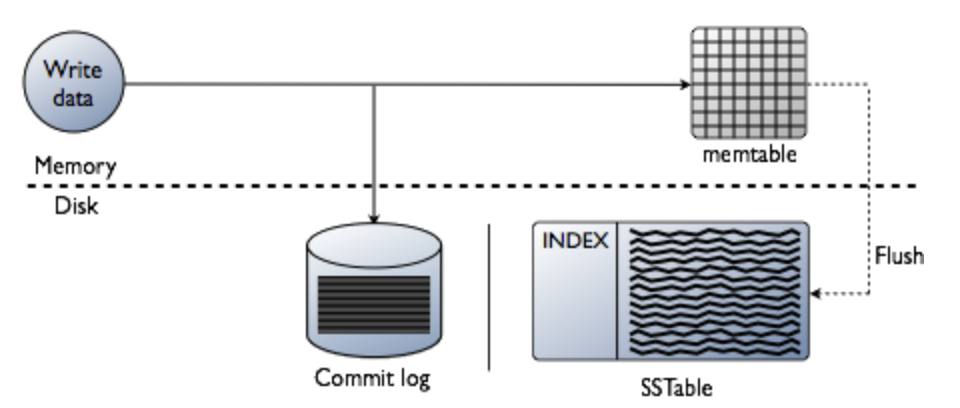
\includegraphics[width=0.8\textwidth]{database_protection-master/assets/casandra.png}
    \caption{Схема записи в Casandra}
    \label{fig:mesh1}
\end{figure}